\documentclass[rnd]{mas_proposal}
% \documentclass[thesis]{mas_proposal}

\usepackage[utf8]{inputenc}
\usepackage{amsmath}
\usepackage{amsfonts}
\usepackage{amssymb}
\usepackage{graphicx}
\usepackage{booktabs}

\title{Variant Effect Prediction for \\ Human Nicotinic Acetylcholine \\ Receptors using Machine Learning}
\author{Hari Krishna Mohan Raj}
\supervisors{Karl Kirschner\\Alexander Hagg\\Prof. Dr. Sebastian Houben}
\date{September 2026}

% \thirdpartylogo{path/to/your/image}

\begin{document}

\maketitle

\pagestyle{plain}

\section{Introduction}

\subsection{Topic of This R\&D Project}

\subsubsection{What nicotinic acetylcholine receptors are and why their variants matter}
Nicotinic acetylcholine receptors (nAChRs) are pentameric ligand-gated
ion channels that mediate fast synaptic transmission at the neuromuscular
junction and throughout the central and peripheral nervous systems. They
are assembled from a repertoire of sixteen subunits ($\alpha$1--$\alpha$7,
$\alpha$9, $\alpha$10, $\beta$1--$\beta$4, $\gamma$, $\delta$, $\varepsilon$).
Missense variants in the genes encoding these subunits give rise to a
spectrum of disorders: congenital myasthenic syndromes (CMS) from
muscle-type receptor mutations, autosomal dominant nocturnal frontal lobe
epilepsy (ADNFLE) from mutations in \emph{CHRNA4} and \emph{CHRNB2}, and a
growing list of neurodevelopmental and psychiatric phenotypes linked to
rare variants in additional subunits \cite{cms_review,schaaf2011}.

The functional consequence of a single amino-acid substitution depends not
only on the chemical nature of the change but on \emph{where} in the receptor
it occurs and \emph{which} subunit carries it. A substitution in the
agonist-binding pocket may alter ligand affinity; a substitution in the M2
pore-lining helix may change channel conductance or ion selectivity; a
substitution in the intracellular loop may affect trafficking to the membrane
or desensitisation kinetics. The same substitution in $\alpha$4 versus
$\alpha$7 can produce opposite phenotypes because the two subunits assemble
into receptors with different stoichiometries and expression profiles.

\subsubsection{The challenges that must be addressed}
\textbf{Must be addressed:}
\begin{itemize}
    \item \textbf{Data scarcity.} The curated dataset contains 717 labelled
    variants, at least an order of magnitude smaller than the millions of
    variants used to train general VEPs(Variant Effect Predictors). Small data amplify overfitting,
    high-variance performance estimates, and limited generalisability to
    subunits not represented in training \cite{cadd,alphamissense}.
    \item \textbf{Label noise and assay heterogeneity.} LOF/GOF labels are
    extracted from studies spanning decades, laboratories, and protocols.
    Two-electrode voltage clamp in \emph{Xenopus} oocytes differs from patch
    clamp in mammalian cells in ways that can flip a marginal LOF/GOF call.
    \item \textbf{Gene leakage in evaluation.} Variants cluster heavily within
    a few subunits (e.g.\ CHRNA1, CHRNA7). A naive random split lets variants
    from the same subunit span train and test, inflating apparent performance.
    Evaluation must group by subunit.
\end{itemize}
\textbf{Nice-to-have:}
\begin{itemize}
    \item \textbf{Cross-species transfer.} Mouse and rat electrophysiology is a
    rich untapped source of labels, but residue numbering differs between
    species and must be corrected by sequence alignment before it can be used.
    \item \textbf{Structural coverage.} Not every subunit has a high-resolution
    cryo-EM structure, and not every position within a solved structure is
    resolved; unmappable positions must be excluded or imputed.
    \item \textbf{The LOF/GOF dichotomy.} A minority of variants show mixed or
    context-dependent effects that a binary label cannot represent.
\end{itemize}

\subsection{Relevance of This R\&D Project}

\subsubsection{Real-world applications}
The main beneficiaries are clinical genomics and the diagnosis of
nAChR-linked channelopathies. A predictor that reports the direction of
effect would help triage variants of uncertain significance (VUS) in
\emph{CHRNA1}, \emph{CHRNB1}, \emph{CHRND}, and \emph{CHRNE} (muscle
subunits implicated in CMS), and in \emph{CHRNA4}, \emph{CHRNB2}, and
\emph{CHRNA2} (neuronal subunits implicated in epilepsy). Because loss of
function (LOF) and gain of function (GOF) demand opposite therapies, a
clinician needs to know the direction, not just whether a variant is
damaging. Beyond the clinic, the curated dataset and the benchmarking
framework are a resource for the broader variant-effect community: a shared,
experimentally labelled nAChR test set on which future methods (protein
language models, structure-based graph networks, and cross-species transfer
approaches) can be compared fairly.

\subsubsection{Concrete numbers}
The scale of the problem is measurable. Fewer than five hundred human nAChR
variants have been experimentally characterised, while tens of thousands of
missense variants per individual await interpretation. A curated dataset of
717 experimentally labelled variants (363 LOF, 190 GOF, 164 no-net-effect)
across all sixteen human subunit genes, assembled from 507 human, 138 rat, and
72 mouse variants, provides the training basis for the project
\cite{mohanraj2026}. The closest published direction-aware system, MissION,
reports ROC-AUC $0.925$ across 47 ion-channel genes but does not model nAChR
subunit identity or pentameric assembly \cite{mission}. Closing the gap between
a generic direction predictor and an nAChR-specific one is what this project
quantifies.

\subsubsection{Why the nAChR-specific choice matters}
A gene-agnostic predictor collapses all subunits into a single model space, so
it cannot express the fact that a substitution's effect depends on which
subunit carries it. Because nAChR subunits assemble into receptors with
different stoichiometries and expression profiles, subunit identity is expected
to be a primary determinant of direction of effect. Pathogenicity scores, for
their part, are trained to separate damaging from benign variants and are not
designed to resolve how a damaging variant alters function. An nAChR-specific,
subunit-aware model is therefore the right level of resolution for this
problem.

\section{Related Work}

\subsection{Survey of Related Work}

\subsubsection{Pathogenicity-only predictors}
SIFT \cite{sift} uses sequence conservation across homologues to flag
substitutions that deviate from the evolutionary norm. PolyPhen-2
\cite{polyphen2} combines sequence conservation with structural features
(surface accessibility, crystallographic B-factor) trained on the HumDiv and
HumVar datasets. CADD \cite{cadd} integrates over sixty genomic annotations
into a single pathogenicity score using a linear-kernel SVM, trained on
$\sim$15M variants. AlphaMissense \cite{alphamissense} leverages AlphaFold
structures and MSA-based conservation to achieve state-of-the-art
proteome-wide pathogenicity prediction, and ESM-1b-based VEPs
\cite{esm1b} apply deep protein language models to the same task. All of these
output a single score where higher means ``more likely pathogenic''; none
distinguishes LOF from GOF.

\subsubsection{Direction-aware predictors}
funNCion \cite{funncion} predicts direction for sodium and calcium channel
variants associated with epilepsy and cardiac arrhythmia, using a random
forest trained on $\sim$800 characterised variants and features spanning
Grantham distance, BLOSUM scores, and intra-protein position. LoGoFunc
\cite{logofunc} performs genome-wide LOF/GOF/neutral prediction using an
ensemble of gradient-boosted trees trained on ClinVar labels. PreMode
\cite{premode} frames mode-of-action prediction as a graph-neural-network
problem over protein structure. MissION \cite{mission} is the closest
precursor: it combines ESM-2 embeddings with structural features (secondary
structure, relative solvent accessibility, per-residue B-factor) to predict
LOF versus GOF across 47 ion-channel genes, reporting ROC-AUC $0.925$.
It demonstrates that structural features complement sequence embeddings for
ion-channel classification, but it aggregates data across diverse channel
families and does not encode nAChR subunit identity or pentameric assembly.

\subsubsection{nAChR structural biology and channelopathy curation}
High-resolution cryo-EM structures of nAChRs \cite{nachr_structure_2021}
provide the structural context (the agonist-binding interface, the M2
pore-lining helix, the M2--M3 linker, and the subunit interfaces) that
determines where a substitution lands and how it perturbs gating. A long
clinical literature on congenital myasthenic syndromes
\cite{cms_review} documents the concrete phenotypes of specific subunits and
the slow-channel versus fast-channel distinction, grounding the LOF/GOF
dichotomy in real mechanisms. AAindex \cite{aaindex} supplies the quantitative
physicochemical descriptors of each amino-acid substitution.

\subsubsection{Cross-species and transfer-learning methods}
Because nAChR electrophysiology is expensive, mouse and rat studies are an
important source of additional labels. Methods for transferring functional
knowledge across species (embedding-based functional equivalence and
network-based gene similarity) offer a principled route to augmenting the
human dataset, provided residue numbering is first corrected by sequence
alignment.

\subsection{Limitation and Deficits in the State of the Art}

\subsubsection{No direction-aware predictor is specific to nAChRs}
funNCion covers Na\textsuperscript{+}/Ca\textsuperscript{2+} channels,
LoGoFunc is genome-wide and gene-agnostic, PreMode is gene-family-agnostic, and
MissION aggregates 47 channel genes including nAChRs but without modelling
subunit identity or pentameric assembly logic \cite{funncion,logofunc,premode,mission}.
None treats the nAChR as a multi-subunit receptor whose direction of effect
depends on which subunit carries the variant.

\subsubsection{Direction of effect is conflated with pathogenicity}
The widely used pathogenicity scores (CADD, AlphaMissense, ESM-1b) are trained
and evaluated on ``damaging versus benign'' and carry little signal for
direction. These tools are optimised to separate damaging from benign
variants, not to resolve how a damaging variant alters function. A direction
predictor must therefore be built and benchmarked on direction labels, rather
than borrowed from pathogenicity tools \cite{esm1b,alphamissense}.

\subsubsection{No shared benchmark or curated nAChR direction dataset exists}
Until this project, there was no publicly curated, experimentally labelled
nAChR dataset with LOF/GOF/no-net-effect labels, and no standard
leave-one-subunit-out protocol against which methods could be compared. Each
prior direction-aware tool reports on its own data and its own splits, making
cross-method comparison impossible \cite{mission,funncion}.

\section{Problem Statement}

\subsection{Deficits I Will Solve}
\begin{enumerate}
    \item \textbf{D1: No nAChR-specific direction predictor.} Build and
    benchmark a predictor whose feature representation and evaluation are
    designed around nAChR subunit identity and pentameric structure.
    \item \textbf{D2: Subunit identity discarded.} Encode subunit identity
    explicitly as a first-class input, and evaluate under a strict
    leave-one-subunit-out protocol that tests generalisation to unseen subunits.
    \item \textbf{D3: Direction conflated with pathogenicity.} Benchmark on
    direction labels only, and quantify how little pathogenicity signals
    contribute to direction, as an explicit finding.
    \item \textbf{D4: No shared dataset or benchmark.} Release the curated
    dataset and the evaluation protocol as a reusable resource for the field.
\end{enumerate}

\subsection{Intended Approach}

\subsubsection{Curated, experimentally labelled dataset}
Assemble a dataset of experimentally characterised nAChR missense variants by
systematic, high-recall mining of primary electrophysiology literature
(PubMed, Europe PMC, UniProt). Each variant is annotated with subunit gene,
wild-type and mutant residue, residue position (canonical, signal-peptide
inclusive numbering), the LOF/GOF/no-net-effect label as stated by the
original authors, the assay type, and the source PMID. Mouse and rat variants
are mapped onto the human numbering frame by sequence alignment before being
combined. The current dataset holds 717 variants (363 LOF, 190 GOF,
164 no-net-effect) across sixteen genes \cite{mohanraj2026}.

\subsubsection{Modelling and rigorous evaluation}
Benchmark a panel of ten classifiers (logistic regression, linear and RBF SVM,
k-NN, Gaussian naive Bayes, MLP, Random Forest, XGBoost, LightGBM, and
CatBoost) under nested cross-validation. The outer loop is
leave-one-subunit-out (StratifiedGroupKFold with the subunit gene as grouping
variable), the strictest test of generalisation to unseen subunits; the inner
loop is stratified 3-fold CV driving Optuna Bayesian hyperparameter
optimisation \cite{optuna}. Performance is reported as macro-F1, Matthews
correlation coefficient, and balanced accuracy, with the three-class task
(LOF/NNE/GOF) as the primary framing and the binary LOF-vs-GOF task as a
secondary framing.

\subsection{How This Approach Addresses Each Deficit}
\begin{enumerate}
    \item \textbf{D1} is solved by designing every stage (features, models, and
    evaluation) around nAChR biology rather than borrowing a gene-agnostic
    pipeline.
    \item \textbf{D2} is solved by encoding subunit identity as an explicit
    input and by the leave-one-subunit-out protocol, which together force the
    model to rely on and generalise across subunit identity.
    \item \textbf{D3} is solved by benchmarking exclusively on direction labels
    and by the ablation analysis that measures how little pathogenicity-oriented
    signals contribute to direction.
    \item \textbf{D4} is solved by releasing the curated dataset, the feature
    pipeline, and the evaluation protocol as an open resource.
\end{enumerate}

\subsection{Evaluation}
The primary metric is macro-averaged F1, which is robust to the LOF-heavy
class imbalance; it is complemented by balanced accuracy and the Matthews
correlation coefficient. Because variants cluster within subunits, all
estimates are produced under leave-one-subunit-out cross-validation, so a model
is scored on its ability to predict direction for a subunit it never saw during
training. The final comparison places the predictor against the published
direction-aware tools (MissION, LoGoFunc, funNCion) on the same nAChR test
folds, and the feature-group ablation attributes performance to individual
feature categories.

\section{Project Plan}

\subsection{Work Packages}
Five work packages decompose the project into concrete steps, each mapped to
one or more of the four deficits.

\begin{enumerate}
    \item[WP1] \textbf{Literature study and curation protocol.} Survey the VEP
    landscape (pathogenicity-only and direction-aware), define the LOF/GOF/NNE
    label criteria, and specify the high-recall search strategy across PubMed,
    Europe PMC, and UniProt.
    \item[WP2] \textbf{Dataset assembly and cross-species alignment.} Execute
    the search, manually curate each paper, and map mouse and rat numbering
    onto the human frame by sequence alignment to grow the dataset beyond the
    current 717 variants.
    \item[WP3] \textbf{Subunit-aware and structural extension.} Add explicit
    subunit conditioning, pentameric interface/pore geometry, and
    conformational features; evaluate graph-neural-network architectures if
    time permits.
    \item[WP4] \textbf{Evaluation against state of the art and ablation.}
    Compare against MissION, LoGoFunc, and funNCion on shared nAChR folds,
    run the feature-group ablation, and produce interpretability analysis
    (feature importance).
    \item[WP5] \textbf{Project report.} Document the dataset, methods, results,
    limitations, and future work, and prepare the final presentation.
\end{enumerate}

\subsection{Milestones}
Milestones mark measurable decision points and the completion of major
activities.
\begin{enumerate}
    \item[M1] Literature review completed; curation protocol and label criteria
    fixed; dataset v1 (717 variants) validated.
    \item[M2] Dataset assembled and cross-species numbering aligned.
    \item[M3] Predictor trained and evaluated under leave-one-subunit-out
    cross-validation.
    \item[M4] Subunit-aware and structural extensions evaluated; ablation
    complete.
    \item[M5] State-of-the-art comparison and interpretability analysis
    complete.
    \item[M6] Report written and submitted.
\end{enumerate}

\subsection{Project Schedule}
The project runs over six months. Figure~\ref{fig:gantt} gives the Gantt chart.
Writing the report is spread across the whole project, not concentrated at the
end.

\begin{figure}[h!]
    \centering
    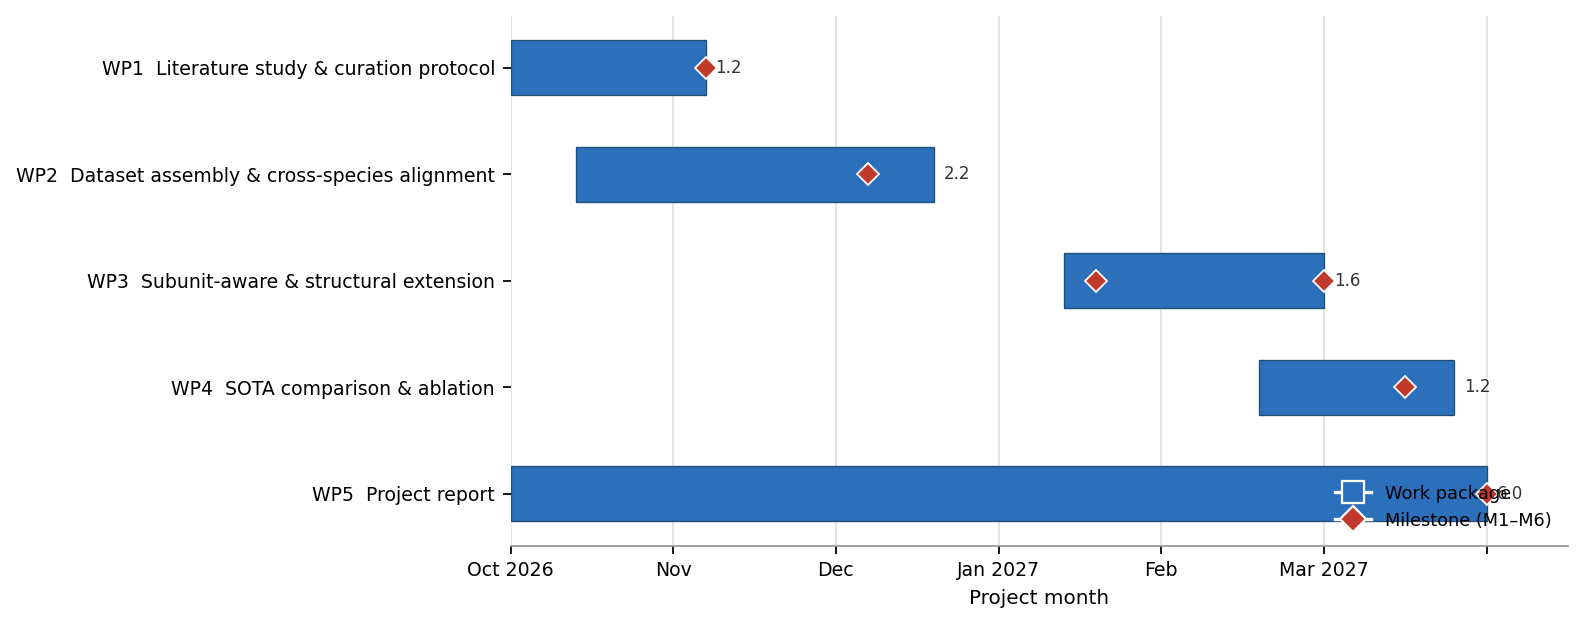
\includegraphics[width=\textwidth]{images/gantt}
    \caption{Gantt chart of the six-month project schedule. The five work
    packages are shown as horizontal bars; the six milestones (M1--M6) are
    marked as diamonds.}
    \label{fig:gantt}
\end{figure}

\subsection{Deliverables}

\subsubsection*{Minimum Viable}
\begin{itemize}
    \item A curated, cleaned dataset of experimentally labelled nAChR missense
    variants (LOF/GOF/no-net-effect) with cross-species numbering mapped to
    the human frame.
    \item A reproducible feature-engineering pipeline for the engineered
    sequence and structural features.
    \item A benchmark of multiple classifiers under leave-one-subunit-out
    nested cross-validation, with results reported.
\end{itemize}

\subsubsection*{Expected}
\begin{itemize}
    \item Subunit-aware modelling, with an ablation that quantifies the
    contribution of subunit identity relative to other feature groups.
    \item A direct comparison against MissION, LoGoFunc, and funNCion on
    shared nAChR test folds.
    \item A feature-group ablation attributing performance to each feature
    category.
\end{itemize}

\subsubsection*{Desired}
\begin{itemize}
    \item Stronger sequence representations evaluated (fine-tuned ESM-2 with
    LoRA; thermostability change $\Delta\Delta G$ from ThermoMPNN or RaSP).
    \item Structural and graph-network features (pentameric interface/pore
    encoding; PreMode-style GNN) evaluated.
    \item A released benchmark (curated dataset plus evaluation protocol), with
    a short report positioning the project for the field.
\end{itemize}

Please note that the final grade will not only depend on the results obtained
in this work, but also on how the results are presented.

\nocite{*}

\bibliographystyle{plainnat}
\bibliography{bibliography}

\end{document}
